\chapter{Implementation}
-How implemented
\section{Approach}
\par The development approach taken focused on the business-logic, or back-end, of the system. From the two main possible development methodologies, Waterfall and Agile, the latter was used. In Waterfall, the devleopment process is a sequential process, where the dvelopment is considered as a sequence of phases that are completed one after the other (cite). In Agile, the focus in adaptive planning, evolutionary development, and continous improvement. The advantage of using an Agile approach over a Waterfall approach is that new features can be mplemented into the system easier. 
\par The most used way of using Agile methodology is through Sprint cycles. These are short development cycles, where a set of features must be implemented, alongside their tests to ensure the correctness of features(discussed in the Testing section). For this project, the cycles combined with the supervisor meetings. Since in them, the new features that were implemented were discussed alongside the new features that were to be implemented in the next cycle. 
\par A clear example of the advantage of this system was when the a new timeline view was suggested. In this new view, rather than having the events row by row, events that occurred during the same time period should be grouped. In addition, events that happened within that time period should be encapsulated by the larger events. This could be implemented in the system, due to the separation of the business logic and the view, and the development approach used. In a Waterfall model, the development is more structured, and thereby it is extremely useful for static requirements, i.e. requirements that will not change. However, in this case it would have caused issues in implementing the new view as it would require going up the Waterfall if the view of the system had already been implemented, or waiting until that step of the waterfall had been reached.
\par While the Agile methodology is mostly used in software development teams, it can be applied to single development projects. Since the structure allows for reviews of features which can be matched with supervisor meetings, and changes in the requirements of the project.
\section{Tools \& Software Libraries}
-development environment
-why used that environment
-software libraries (include an example use)
-why
\par The development environment of the project is a 64-bit Windows 10 machine, with a Intel Core i7-6700HQ CPU at 2.60GHz and 16.0GB of Random Access Memory (RAM). It includes a Java Intelligent Development Environment (IDE), with Git for version-control, and Gradle for dependency management. 
\par The use of verion-control allows development of features separata of working code, and only adding them to the working version if the required tests pass. It should be noted that Git flow was used. This involves having a develop branch with the newest working features of the system. The master branch will only contain the lastest fully implemented working version of the product. This allows for mistakes in development to be rolled-back to a state where the system worked correctly.
\par Gradle allows for libraries to be regarded as dependencies of the project. Such that when the system is ran on a separate machine, it will retrieve all the missing libaries used in the project before compiling and running the program. This allows for the system to be shared to other users, without having to include the libraries with the distribution of the code, as the required libraries and the version will be downloaded to the users system when they run the command: \makebox[\textwidth]{ \textbf{gradlew run}.} Where the gradlew is a wrapper for gradle, such that the user does not even have to have Gradle in their system to launch the system. This provides obvious advantages of portability and general use.
\par As mentioned in the Background chapter, multiple libraries exist to aid the task of Natural Language Processing. These are especially needed for the Named Entity Recognition(NER) and Text Summary task. As an NER annotator will tag certain words, or collection of words into predefined categories such as People, Companies, Locations, and Money. This is extremely useful for the task of identifying dates in sentences, and the subjects described in the sentences. In addition, these tools can aid in the tagging of words using the P.O.S Treebank, which is required for the implementation of the Hedge-Trimmer algorithm \cite{dorrzajicschwartz2003} for headline generation (i.e. summary of a sentence). The main advantage of using libraries for this task over developing these annotators, is that building such an annotator requires multiple developers and many years of work. This can be seen from the 	release history of the StanfordCoreNLP tool which intially released in 2010, but still in October 2016 new releases have been made\footnote{\url{http://stanfordnlp.github.io/CoreNLP/history.html}}. The main two NLP tools are Apache's OpenNLP\footnote{\url{https://opennlp.apache.org/}} and Stanford's CoreNLP\footnote{\url{http://stanfordnlp.github.io/CoreNLP/index.html}}. For this project the Stanford's tool was used in the implementation, as it provides an extended documentation and examples of using their tools, along with specific sections for each of their annotators. The Stanford tool is the main library used throughout the project, as the project is reliant on its NER and POS annotators (cite the stanford annotators). It comes with models, that are loaded during the initialisation of the system. These models are used in the annotators to determine whether certain words fall in predefined categories, or which POS tag should be given to them, through the use of statistics that are based on the models. 
\par As the two main NLP libraries available are Java implementations, the decision was made to build the system in that language. It would be problematic to build the system in a different language to its libraries, as it would require to make the two programming languages communicate with each other, which can cause unpredictable problems in the development and execution of the system.
\par Additional libraries in the development include JUnit for Unit testing. This allows for features of the system to be developed and for them to be tested for correctness. With the addition of the Git flow, when new features are developed, they are done on a separate branch. Before they are joined to the latest working version of the system the tests for other features and the current developed feature can be ran, thereby ensuring that the system is still working as expected even with the new feature. Unit testing allows for part of a system to be ran, and then to produce a result and compare it to an expected result. The test would then pass if the results match. Testing will be further discussed in one of the following sections.
\par Libraries for text extraction of .pdf and .docx file types are required, as the enconding of these files is not in a plain text model. Therefore the Apache POI\footnote{\url{https://poi.apache.org/}} and the Apache PDFBox\footnote{\url{https://pdfbox.apache.org/}} are used. In addition to text extraction, the PDFBox library along with the Apache Commons library allows the creation of PDFs (with text wrapping), which is required to save the timeline as a PDF. The Google GSON\footnote{\url{https://github.com/google/gson}} library is used for the creation of JSONs, which is required to produce an intermediate JSON of the timeline. The RichTextFX\footnote{\url{https://github.com/TomasMikula/RichTextFX}} library along with JavaFX are used to build the graphical interface of the system. All of the libraries included are provided with licenses that allow its use in systems, along as the system is made publicly available, which will be done as the resulting system will be open-source.

\section{Issues}
\par Two main issues arised during the implementation of the system. The creation of exact dates for named  entity dates and the creation of a encapsulated timeline. In addition, a minor issue in the system is input of documents that are grammatically incorrect.
\subsection{Named Entity Recognition (NER) of Dates}
\par The StanfordCoreNLP tool, allows the resolution of temporal expressions. To explain this, an example is presented. For example, the Stanford tool allows for reference dates be used when a document is processed. When the tool tags a temporal expression as DATE, it allows for this temporal expression to be normalized. The annotator treats each word in the sentence as a mention. To identify it's named entity recognition tag, the following is done on the mention: 
\makebox[\textwidth]{\textbf{mention.get(CoreAnnotations.NamedEntityTagAnnotation.class)}.}
If it is a temporal expression that was tagged, the result of the operation is a String DATE (to identify it as a date). Thus, from the mention, it can be normalized using: \par
\makebox[\textwidth]{\textbf{mention.get(CoreAnnotations.NormalizedNamedEntityTagAnnotation.class)}.}
The Stanford tool will attempt to produce a date in the ISO 8601\footnote{\url{https://www.cl.cam.ac.uk/~mgk25/iso-time.html}} format. As can be seen from the format, it can produce exact dates of the type dd-MM-yyyy. Where dd is an integer value from 1 to 31, MM is the month as an integer value from 1 to 12, and yyyy the year. In addition, if BC dates are used, at the start of the normalized result a '-' is added. Using the ISO standard, a method was written to process these dates. However, in addition to the possible dates given by the ISO standard, Stanford builds on top of the standard, producing 3 additional Date normalizations.
\par The normalizations refer to temporal expressions that are ambigious even with a reference point. For example, the temporal expression "now" would produce a normalized NER: "PRESENT\textunderscore REF", i.e. a reference to the present moment. For a temporal expression that refers to the past, e.g. "...they once used to...", "once" would be normalized to "PAST\textunderscore REF", i.e. a reference to the past of this moment. For a temporal expression that refers to the future, e.g. "In the future..., "future" would be normalized to "FUTURE\textunderscore REF", i.e. a reference to the future after this moment. The issue with these normalizations is that the do not allow for the comparison of events used to sort them, as the start and end dates of events cannot be compared. To allow for comparison, the most possible general dates for these references are derived. Since a "PRESENT\textunderscore REF" refers to the present moment, it can be deducted that it represents the moment in which the text was written in, as that is the time context in which the author wrote it in. Thereby, the decision was made to produce as a general date for "PRESENT\textunderscore REF" the reference point provided by the user. Since the reference point is supposed to be the date in which the text was written in, it would be appropriate to link a reference of the present moment to it. The user can change the reference point to when-ever they would like not just the assumed date of the written document, but a present reference should match the base date used by the system to determine all other ambigious dates. For "PAST\textunderscore REF" and "FUTURE\textunderscore REF" a range of dates is used, i.e. a start and end date. For the former, the start date of the era is used, i.e. 01-01-0001, and a end date to the reference point. Since it can be determined that a ambigious mention of the past would fall anywhere within that time period, however an exact determination cannot be made as the temporal expression is not precise enough. For the latter, the start date is the present moment, i.e. the base date, and the end date is the last possible allowable date in the system, i.e. 31-12-9999. Since it would be appropriate for a mention of the future would refer to a moment from now (i.e. the present moment in which the text is presumed to be written in), up until the end of times. However as a limitation to our system, the end of times is considered the date 31-12-9999. This detection part of the normalized NER for Dates is presented as a snippet of the method that produces the exact dates from Normalized NER dates (see Figure \ref{fig:refCode}).
\begin{figure}[H]
\begin{lstlisting}
private ArrayList<Date> getDate(String date) {
	...
	/* Set up variables for processing */
	if (onlyPastRefPattern.matcher(date).matches()) {
            //past so make range from 0001-01-01 -> base date (range)
            if (yearMonthDayPattern.matcher(baseDate).matches()) {
                //base date has the format yyyy-MM-dd
               /*split it and set the values in date1,month1, year1 of 
		the start year 01-01-0001*/
		/*and the end date values of date2, month2, year2 
		to the base date data*/
		...
            }
        } else if (onlyPresentRefPattern.matcher(date).matches()) {
            if (yearMonthDayPattern.matcher(baseDate).matches()) {
                //base date has the format yyyy-MM-dd
		/*set day1,month1,year1 to the data in the base
		 date data*/
		...
            }
        } else if (onlyFutureRefPattern.matcher(date).matches()) {
            if (yearMonthDayPattern.matcher(baseDate).matches()) {
		//set the day1,month1,year1 to the base date data
            }
           //set year2,month2,day2 to the end year 31-12-9999
        }
	...
	/* date1,date2,month1,month2,year1,year2 are 
	then used appropriately to generate dates used 
	for the event that holds this Timeline Date */
}
\end{lstlisting}
\caption{Part of the Implementation of Resolution of Normalized NER Dates}
\label{fig:refCode}
\end{figure}
\subsection{Encapsulated Timeline View}
\par The initial representation of the events was a traditional timeline (see Figure \ref{fig:traditionalView}). This view is effective when the events are on separate time periods, as it presents them one after the other in a sequence. However, when there are multiple events that occur during the same time period, they still appear one after the other. The issue is that unless the user specifically looks at the dates associated to the event, it will look at a first glance as events occuring in different time periods. This clearly violates the visibility objective of the user-interface of the system. A solution to this issue is to provide two views, the traditional timeline view which is effective at displaying events that have disjoint dates. The other view, is one where dates encapsulalte other dates, and hold the events that occur in that time period. For example, if there is more than one event that occurs on the "25-01-2017", then isntead of listing them both of these events are below the same date. This canthey cause a "bin-placing" problem. This where there are a set of bins, or in this case a set of graphical events, and they need to fit in a finite area(cite), in this case a box of certain width and height. However, this problem can be avoided through the use of scrollbars, which provides a container of infinite height, thereby all the bins (graphical representation of events) can be placed. This view has been called the "Range View". However, producing this view, requires placing the Results (the events of a set of documents) in Ranges (a data structure that can have one date, or a start and end date). The theory was discussed in the Design Chapter.
\begin{figure}[H]
\caption{Screenshot of the Traditional View of the Timeline of Events}
\label{fig:traditionalView}
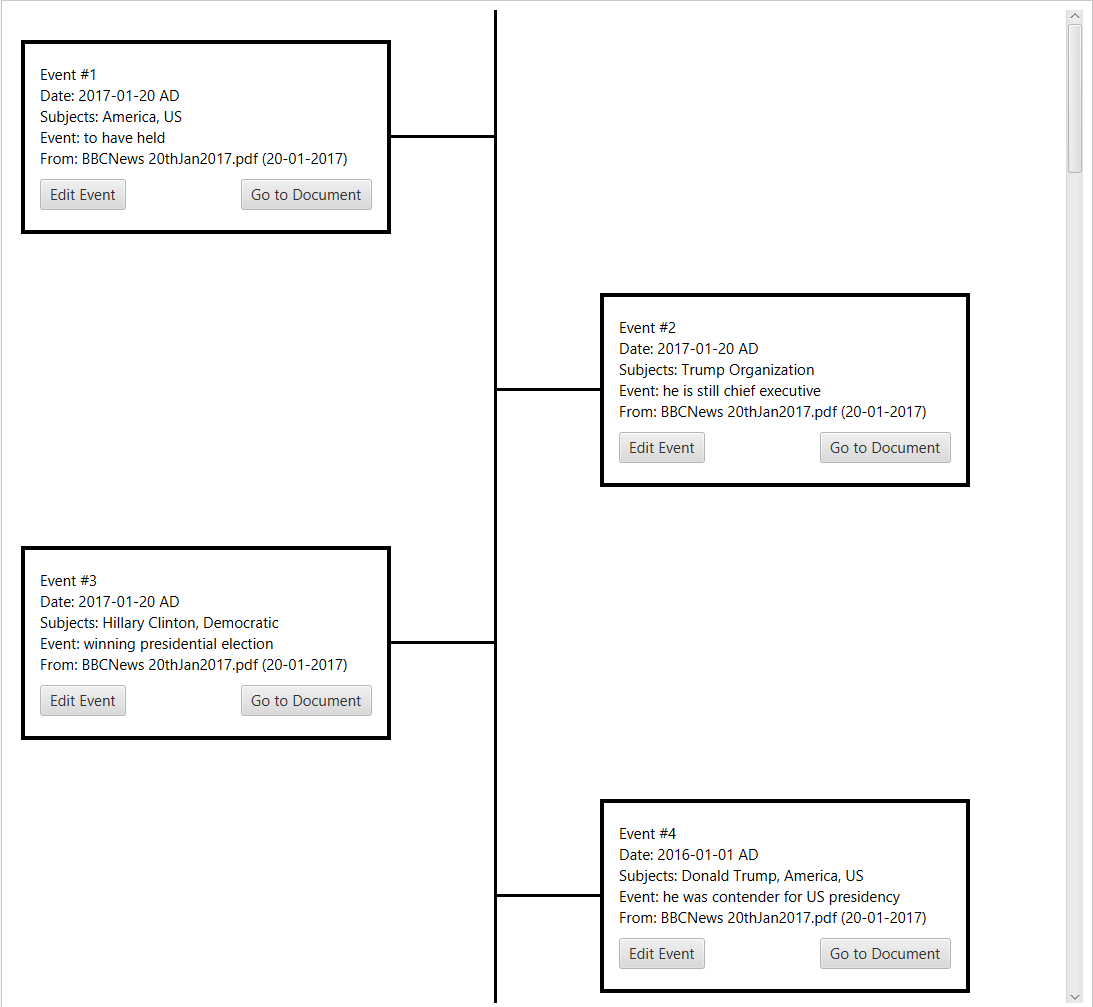
\includegraphics[width=\linewidth]{traditionalView.png}
\centering
\end{figure}
\par The theory behind the Range View, is having a list of Ranges, where each Range is a root node of a Tree of Ranges. Where each Range may hold zero or more Results (i.e. events), and a set of children Ranges (zero or more). When the timeline needs to be produced, the list of Roots is iterated over, assuming the list is of Roots has been sorted in the order of the start date, for each a GridPane is made. A GridPane is a layout which consists of rows and columns that can contain subviews (where a subview is a view, i.e. a graphical component). In the first column of the of the layout, the current Range's data is placed (i.e. the date(s) and the Results held), and in the second column the layouts of the child Ranges is recursively made. The algorithm is presented in Figure \ref{alg:rangeLayout}, it is done for each root Range in the list of Ranges to be created.
\begin{algorithm}[H]
\underline{function getRangeLayout(list l)\; }
\SetKwInOut{Input}{Input}
\SetKwInOut{Output}{Output}
\Input{A list of Ranges, of size $n$, to add in the first column}
\Output{a layout that encapsulates the Ranges passed in the input, and their child Ranges}
GridPane toReturn\;
toReturn set the number of rows to the size of the input\;
toReturn set the number of columns $:= 2$\;
\For{i $:=$ 0 $\shortrightarrow$ n}{
	Range $:=$ input list at $i$\;
	set up layout for this Range, and set it in toReturn at position $(i,0)$\;
	set its column span at $(i,0)$ to remaining\;
	get layout for the children of this Range $:=$ getRangeLayout(range.children)\;
	set this layout in toReturn at position $(i,1)$\;
}
return toReturn\;
\caption{Pseudo-Code of the Recursive Production of the Range Layout}
\label{alg:rangeLayout}
\end{algorithm}
\par The full implementation can be found in the Appendix. In the implementation, it was deceided to include 3 columns, to have a separator between a Range and its children Ranges, to improve the visibility of the system. Allowing the user to differentiate a Range and its child Ranges, and thereby differentiate the Results they hold. The individual layouts of Range is the listing of the Results in that Range (i.e. in the time period of that Range), and the date or start and end date for that Range. An example look of the Range View can be found in Figure \ref{fig:rangeView}.
\begin{figure}[H]
\caption{Screenshot of the Range View of the Timeline of Events}
\label{fig:rangeView}
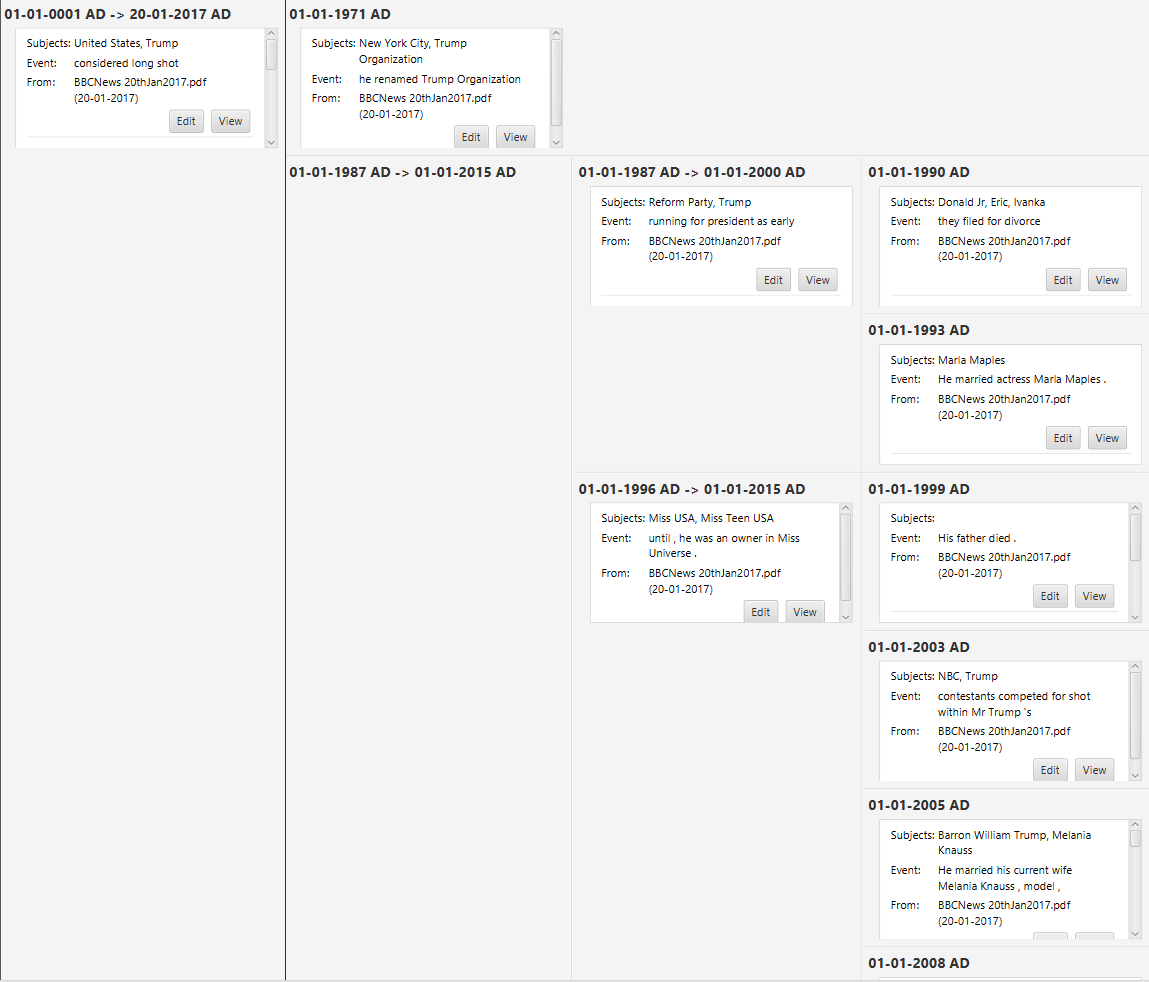
\includegraphics[width=\linewidth]{rangeView.png}
\centering
\end{figure}
\subsection{Incorrect Input Documents}

-ner dates (explain, then present how to solve it through examples of code)
-new timeline view (present how to solve it through examples of code)
-minor issue of incorrect text
\section{Testing}
\section{UI}
\section{Algorithms}
-main algorithms: for building events, building ranges, pdf save, json save, processing files
